\subsubsection{Actividad 2 lab 2}
%*********************

\begin{frame}{Actvidad 2 lab 2}
\begin{figure}[H]
\begin{flushleft}
\item{Realizar un diagrama de  bloques que  muestre los diferentes tipos de  ruidos, $(Gaussian, Laplacian, Impulse \hspace{0.15cm} and  \hspace{0.15cm} Uniform)$ y sus  propiedades .}\\
\end{flushleft}
	

	

\begin{center}
\centering
\includegraphics[width=\textwidth, height=0.58\textwidth]{parte1/lab2/pdf/lab2_18.pdf}
\end{center}
\end{figure}
\end{frame}
%--------------------------------


\begin{frame}

\frametitle{\underline{\textbf{Pistas para la actividad}}}

Las pistas son:
\begin{enumerate}[1.]

\item {Repasar los bloques utilizados en la segunda  guía "Osciloscopio y FFT".}\\
\item {Debe existir un WX GUI Slider  para la Amplitud del  ruido, la  amplitud de  la señal, y la frecuencia.}\\
\item {debe existir un WX GUI Notebook para ver cada  señal  por  separado.}\\
\item {Coherencia entre los tipos de dato entre bloques.}\\


\end{enumerate}
\end{frame}
